%\documentclass{beamer}
%\usetheme{Pittsburgh}
\documentclass{scrartcl}

\usepackage[utf8]{inputenc}
\usepackage{default}
\usepackage[procnames]{listings}
\usepackage{graphicx}
\usepackage{adjustbox}
%\usepackage[toc,page]{appendix}
\usepackage{caption}
\usepackage{hyperref}
\usepackage{color}
%\usepackage{csvsimple}
\usepackage{float}
%\usepackage[T1]{fontenc}



%Bibliogrpahy?
%\usepackage{bibentry}
%\nobibliography*
%\bibentry{ }


%Python
\definecolor{keywords}{RGB}{255,0,90}
\definecolor{comments}{RGB}{0,0,113}
\definecolor{red}{RGB}{160,0,0}
\definecolor{green}{RGB}{0,150,0}
\lstset{language=Python,
    basicstyle=\ttfamily\scriptsize,
    keywordstyle=\color{keywords},
    commentstyle=\color{comments},
    stringstyle=\color{red},
    identifierstyle=\color{green},
    breaklines = true,
    columns=fullflexible,
    %Numbering and tabs
    %numbers=left,
    %numberstyle=\tiny\color{gray},
    %stepnumber=2,
    %numbersep=1em,
    tabsize=4,
    showspaces=false,
    showstringspaces=false}

\begin{document}

\title{Learning and Adaptivity}
\subtitle{Report No. 4}
\author{
  \href{daiem.ali@smail.inf.h-brs.de}{Ali, Daiem}: \href{https://github.com/daiemna}{github.com/daiemna}\\
  \href{christophe.quignon@smail.inf.h-brs.de}{Quignon, Christophe}:\href{https://github.com/ChrisQuignon}{github.com/ChrisQuignon}
  %Familyname, Name
}
\date{\today}


\maketitle

%TODO: add abstract and conclusion
%labels (or zero)
%references (or zero)
%remove scaffolding code


\begin{abstract}
\textbf{Abstract:}
This week we took an in depth look at the parameters of the prediction algorithm and tested several possibilities to get an estimator for their use. The test was not exhaustive, because a full run on all possible permutation of all parameters would take far too long. Instead we reason about which subsets of parameters to test with what values. We varied the input features, the frame sizes of the input and output frames as well as the number of samples of sets of input/output frames. 
%TODO we conluded...
\end{abstract}

\section{Parameter Test}
\label{sec:parameter}
After the analysis of the sliding window and the time-shift we have several parameters to tune. For now, the parameters of the random forest regressor are left as their defaults:
\begin{lstlisting}[language=Python]
class sklearn.ensemble.RandomForestRegressor(n_estimators=10, criterion='mse', max_depth=None, min_samples_split=2, min_samples_leaf=1, min_weight_fraction_leaf=0.0, max_features='auto', max_leaf_nodes=None, bootstrap=True, oob_score=False, n_jobs=1, random_state=None, verbose=0, warm_start=False)
\end{lstlisting}

only  the n\_jobs are adjusted to minimize computing time.\\
We spent some time to adjust and tune the parameters of our own function, that mainly handle sub-sampling and the time window. The function call as of now is:


\begin{lstlisting}[language=Python]
def wrapper(df, validation_delta, timedelta_input, timedelta_output, to_predict, input_sampling, output_sampling, stepwidth):
    """Wrapper for a complete prediction run on a given dataframe df"""

    print 'Learning:'
    print 'Input frame: ', timedelta_input
    print "Input sampling: ", input_sampling
    print 'Output frame: ', timedelta_output
    print "Output sampling: ", output_sampling
    print 'Stepwidth: ', stepwidth
    print 'Features to learn: ', helper.translate(to_predict)
    ...
\end{lstlisting}

And the parameters are discussed in detail in the following subsections.


\subsection{Input/ output features (to predict)}
\label{sec_1}
Following figure \ref{fig:feat_remove} shows the effect of removing each features on the error. Each feature was removed from the feature list and a model was trained using remaining features, then the test was conducted giving us the effect of removing each feature from the dataset. we can see in the figure \ref{fig:feat_remove} that precipitation and volumetric-flow affects the prediction error insignificantly so, an argument can be made to remove these features without the lose of information.
\begin{figure}[H]
  %\raggedleft
  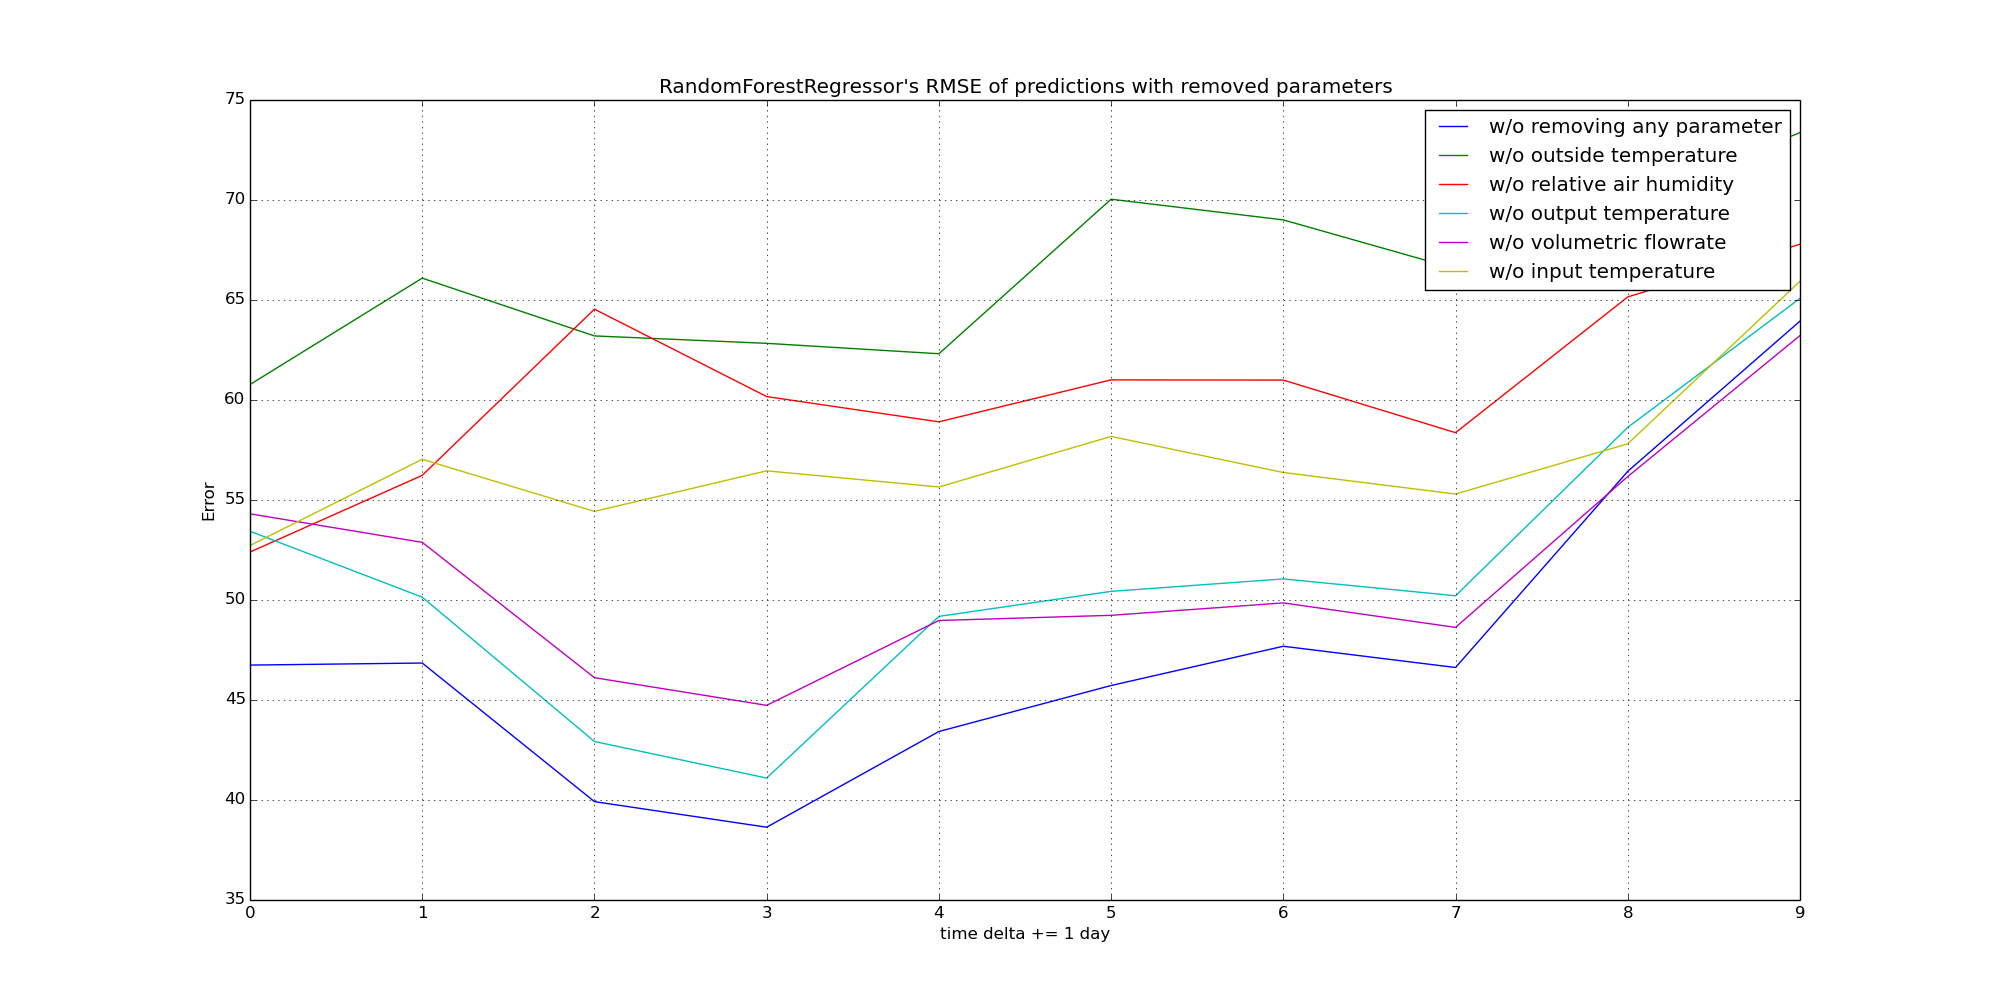
\includegraphics[width=1.2\linewidth]{../../img/RandomForestRegressor_day_error_without_some_params.png}
  \caption{Effect of removal of a features from data.}
  \label{fig:feat_remove}
\end{figure}

\subsection{Training/ validation sets}
\label{sec_2}
As with every learning algorithm, it is necessary to define some of the known input/ output pairs to validate the success of the algorithm. This is done with the validation\_delta parameter that define what time-range is cut off the complete set for validation. As the precedent reports showed, the prediction accuracy of more than than three days significantly drops. Thus we choose a validation set of 7 days, which leaves us with 235 days of training data.
%Validation set is 7 days, rest is training
%As analysed before

\subsection{Input/ output frames}
\label{sec_3:}
The size of the input and output frames are mainly defined by the analysis in the last report which describes the optimal time-shift. The smallest optimal time-shift was a few minutes and the largest optimal time-shift for features that are arguably correlated was around 4 hours. Thus we chose to test input frame sizes of 3, 4, 6, 12 and 24 hours. The output frame size is defined by the problem formulation to be around 3 hours. 
%Input: 3, 4, 5, 6 hours

\subsection{Sampling}
\label{sec_4:}
%more samples -> higher precision
We can sub-sample the input and the output separately. Thus it is possible to look for an optimal trade-off between fast learning time (low sampling) and accuracy (high precision). Once we determined a good set of the other parameters we can just maximize the sampling.

\subsubsection{Training set}
\label{sec_5:}
The sampling of the training set is defined by the minimal time delta between two samples of input and output frames. Thus it defines how many samples we have in total. Here the argument for more information with a higher sampling holds true, but we also have a "natural" sampling of one sample per day. Thus the parameter was tested with 10 minutes and 1 day.

\subsubsection{Input frame}
\label{sec_7:}
We expect that a higher input sampling only affect the outcome positively and thus left this parameter untouched for the parameter test run and set to 10 minutes.

\subsubsection{Output frame}
\label{sec_8:}
The output sampling is likely to affect the accuracy because with more samples to predict it is more likely to miss their values. However it is part of the problem definition to define an acceptable prediction sample rate. We set it to 10 minutes.

\section{Data}
%append the data
\begin{table}[htbp]
\centering
\caption{Overview of the varied parameter, ordered by score.}
\begin{tabular}{r||r|r|r|r}
score & timedelta\_input & timedelta\_output & stepwidth & runtime \\ \hline\hline
-71.00 & 03:00:00 & 03:00:00 & 24:00:00 & 00:00:02 \\ \hline
-3.46 & 04:00:00 & 03:00:00 & 24:00:00 & 00:00:02 \\ \hline
-0.49 & 06:00:00 & 03:00:00 & 24:00:00 & 00:00:02 \\ \hline
0.14 & 12:00:00 & 03:00:00 & 24:00:00 & 00:00:05 \\ \hline
0.47 & 03:00:00 & 03:00:00 & 00:10:00 & 00:03:43 \\ \hline
0.49 & 04:00:00 & 03:00:00 & 00:10:00 & 00:04:20 \\ \hline
0.50 & 06:00:00 & 03:00:00 & 00:10:00 & 00:05:35 \\ \hline
0.54 & 12:00:00 & 03:00:00 & 00:10:00 & 00:09:55 \\ \hline
0.63 & 24:00:00 & 03:00:00 & 00:10:00 & 00:26:53 \\ \hline
0.94 & 24:00:00 & 03:00:00 & 24:00:00 & 00:00:04 \\ 
\end{tabular}
\label{tab:testrun}
\end{table}

\section{Conclusion} 
%TODO Daiem Conclusion

The outcome as seen in table \ref{tab:testrun} has a great variety of scores but also show two trends:

\begin{itemize}
\item A larger input frame has a higher score
\item More samples results in higher training time.
\end{itemize}

The second was as expected, but a full day input size at 10 minute resolution run in 30 minutes is still expectable. To extend the input beyond one day seems unnecessary since it can be argued that system input of one day before can not affect the output. On the other hand, the score of 0.94 has to be taken with a grain of salt, since it is very coarse grained. It is also to mention, that every run was annually concluded once which leaves us with the possibility of a randomly good or bad outcome.



%BIBLIOGRPAHY?
\bibliographystyle{plain}%amsalpha
\bibliography{bib.bib}
%\bibentry{}

%\begin{appendix}
%\section{}

%\end{appendix}


%COPY AND PASTE FROM HERE

%\begin{enumerate}
% \item
%\end{enumerate}

%\href{link}{text}

%\begin[Language=Python]{lstlisting}
%#PYTHON CODE HERE
%\end{lstlisting}

%\lstinputlisting[language=Python]{	}

%\csvautotabular[separator=semicolon]{data.csv}


%\begin{figure}[H]
%  \centering
%  \includegraphics[width=0.5\linewidth]{../img/	}
%  %\caption{}
%  %\label{fig:}
%\end{figure}
%PUT UNITS ON THE FIGURES

\end{document}
